\section{Physarum-based Metaheuristic}
\label{section:algorithm_metaheuristic}

The final experience with the theoretical physarum machine was rather dissapointing, however we still wanted to make it useful in practice. We thought of simulating \textit{Physarum polycephalum}, hoping to lower execution time for the naive algorithm. Instead we propose a new algorithm designed from the ground up, which is inspired by the observed behaviour of the slime mould. While the algorithm was created for solving Quadratic Assignment Problem, it is an universal metaheuristic which can be applied to a number of optimisation problems.


\subsection{Algorithm overview}

The algorithm can be divided into three distinct phases: exploration, crawling and merging. These phases are executed sequentially in a loop, until stop condition is satisfied. General overview of the algorithm can be seen in a pseudocode \ref{algorithm:m_general}. 

\begin{algorithm}[H]
  \KwData{optimisation problem with neighbourhood definition}
  \KwResult{approximated result}
  \BlankLine

  environment $\leftarrow$ initialize\_environment(problem)\;
  colony $\leftarrow$ initialize\_colony(environment)\;

  \Repeat{${\neg}colony.alive \lor {\neg}experiment.next$}{
    \For{$plasmodium \in colony$}{
      plasmodium.explore()\;
      plasmodium.crawl()\;
    }
    colony.merge()\;
  }

  \Return{colony.largest}\;

  \caption{Overview of physarum-based metaheuristic}
  \label{algorithm:m_general}
\end{algorithm}

Initialization of the environment includes sampling of solutions space: $k$ random assignments are taken, for each of them a cost is computed (pseudocode \ref{algorithm:m_env_initialization}). An assignment with the smallest cost is saved as an exemplar for the further calibration.  The colony of ``virtual physarum'' is put on best $l$ out of $k$ samples (pseudocode \ref{algorithm:m_colony_initialization}).

\begin{algorithm}
  \KwData{optimisation problem}
  \KwResult{list of samples}
  \BlankLine

  solutions $\leftarrow$ \{\}\;
  \For{$i \leftarrow 0$ \KwTo $k$}{
    solutions $\leftarrow$ solutions $\cup$ \{random\_solution()\}\;
  }

  sorted\_solutions $\leftarrow$ sort(solutions, problem.cost)\;
  environment.best\_cost $\leftarrow$ problem.cost(sorted\_solutions.first)\;
  
  \Return{sorted\_solutions}\;

  \caption{Initialization of environment}
  \label{algorithm:m_env_initialization}
\end{algorithm}

\begin{algorithm}
  \KwData{environment with sampled solutions}
  \KwResult{set of virtual physarum}
  \BlankLine

  colony $\leftarrow$ \{\}\;
  \For{$i \leftarrow 0$ \KwTo $l$}{
    plasmodium $\leftarrow$ create\_plasmodium(environment.samples[i])\;
    colony $\leftarrow$ colony $\cup$ \{plasmodium\}\;
  }
  \Return{colony}\;

  \caption{Initialization of colony}
  \label{algorithm:m_colony_initialization}
\end{algorithm}

Simulation stops when plasmodia crawl no more (are dead of lacking energy) or given number of iterations or time has been exceeded. A result of the optimization can be obtained as the solution with the smallest cost which is occupied by the virtual physarum at the end of the simulation.


\subsection{Environment}

The naive algorithm assumed an uniform distribution of food sources which are inversely proportional to the cost of a solution, however there is no such direcct need in our metaheuristic solution. In a similar manner solutions are represented as virtual food sources, but they are generated dynamically --- virtual food consume no memory unless they are visited by plasmodium. ``Nutritional energy" is calculated dynamically when a food is visited as follows: 

% TODO maybe just frac squared???
\begin{equation}
  E_{solution} = a \cdot q^{\frac{calibrated\_cost}{cost(solution)}} + {\Delta}E_{solution}
  \label{equation:m_e_solution}
\end{equation}

Where $calibrated_{cost}$ is a cost of the minimal solution obtained via the initial sampling process, $a > 0$ is a scaling factor, $q > 1$ is an exponentiation base. ${\Delta}E_{solution}$ is already consumed energy from a corresponding $solution$. At the start each ${\Delta}E_{solution}$ is equal $0$, so there is no need of storing such information, but as plasmodium explores and crawls ${\Delta}E_{solution}$ is updated, taking at most $O(n!)$ memory if every solution would be explored.

The algorithm defines a neighbourhood for Quadratic Assignment Problem as single pair swap, giving $\frac{n\cdot(n-1)}{2}$ possible neighbours for each assignment. However, instead of a deterministic generation of the neighbourhood, a stochastic one is used --- the neighbour solution is created by swapping two random positions from the given assignment. Within this environment lives a colony of virtual plasmodia --- $l$ different plasmodia are placed on different food sources selected from the initial sampling (pseudocode \ref{algorithm:m_colony_initialization}). 

\subsection{Virtual plasmodium}

A plasmodium is an active state of \textit{Physarum polycephalum}, in laboratory it moves on an agar substrate foraging for food, usually the oatmeal. It feeds by covering multiple food sources with its body and transfers nutrients to its distant parts.

Virtual plasmodium is modelled after biological one: it feeds on virtual food, which provides energy required for further exploration and movement. The energy is essential for keeping the plasmodium active --- most of it is used for an exploration phase, while the rest is used for the actual movement to the other food sources. Each virtual plasmodium is created with some initial energy $E_{initial}$ motivating initial exploration (still changing ${\Delta}E_{plasmodium}$, but not changing ${\Delta}E_{solution}$). After exploration it can crawl to some of explored food sources and exploit every source of energy it occupies --- the plasmodium has that much energy as much food is available under its body (plus some extra initial energy):

\begin{equation}
  E_{plasmodium} = E_{initial} + {\Delta}E_{plasmodium} + \sum\limits_{solution \in plasmodium} E_{solution}
\end{equation}

\noindent If no energy is left ($E_{plasmodium}$ is equal zero), the plasmodium is considered dead.


\subsubsection{Exploration phase}

The plasmodium in the exploration phase browses the neighbourhood, so new food sources can be found (pseudocode \ref{algorithm:m_exploration}). For every already occupied food source, a neighbour is generated by swapping two randomly chosen assignments. Such neighbour solution is added to a frontier, which is an analogy to slime mould's head. Each visit consumes parametrized $E_{explore}$ energy. This phase is repeated as long as there is enough energy left for crawling to another solution $E_{crawl}$. Exploration consumes pool of $E_{initial}$ energy, when none is left, energy from the food sources is used, effectively decreasing $E_{solution}$ available within the environment.

\begin{algorithm}
  \KwData{plasmodium placed within environment}
  \KwResult{solutions frontier}
  \BlankLine

  frontier $\leftarrow$ \{\}\;
  \Repeat{$E_{crawl} \geq E_{plasmodium}$}{
    \For{$solution \in plasmodium$}{
      next\_solution $\leftarrow$ environment.neighbour(solution)\;
      frontier $\leftarrow$ frontier $\cup$ \{next\_solution\}\;

      \uIf{$E_{initial} \geq |{\Delta}E_{plasmodium}| + E_{explore}$}{
        ${\Delta}E_{plasmodium} \leftarrow {\Delta}E_{plasmodium} - E_{explore}$\;
      }
      \Else{
        ${\Delta}E_{solution} \leftarrow {\Delta}E_{solution} - E_{explore}$\;
      }
    }
  }

  \Return{frontier}\;

  \caption{Plasmodial exploration phase}
  \label{algorithm:m_exploration}
\end{algorithm}

The plasmodium in exploration phase simply selects candidate solutions (frontier) for the further optimization. Physarum can occupy many food sources, representing this way a trail of previously tested solutions --- when choosing a neighbour it tries to avoid suspension in a local minimum as it can explore historic neighbourhoods.

\subsubsection{Crawling phase}

In a crawling phase, the plasmodium onto new food sources. Food sources discovered in exploration phase as a frontier are sorted by their energetic value. If none has been found, plasmodium is considered to be dead. Crawling is split into two parts --- adding new food source and removal of inefficient food sources (pseudocode \ref{algorithm:m_crawling}). Plasmodium crawls onto the most energetic food source in a frontier only if its energy recompensates energy of discovering and crawling (when plasmodium creeps onto a new food source it uses $E_{crawl}$ energy). 

Plasmodium leaves previously occupied food sources when the worst solution in the frontier carries more energy than considered food source (even after including $E_{crawl}$). This behaviour controls size of plasmodial body, which in fact could be treated as a history of solutions. Crawling phase can be considered asymmetric by the results --- it adds at most a single food source, but can result in a removal of multiple food sources from the body.

\begin{algorithm}
  \KwData{plasmodium placed within environment}
  \KwResult{new state of plasmodium}
  \BlankLine

  \If{$frontier = \emptyset$}{
    \Return{dead}\;
  }

  sorted\_frontier $\leftarrow$ sort(frontier, $E_{solution}$)\;

  best\_solution $\leftarrow$ front(sorted\_frontier)\;
  worst\_solution $\leftarrow$ back(sorted\_frontier)\;

  \If{$E_{best\_solution} > E_{crawl} + E_{explore}$}{

    \uIf{$E_{initial} \geq |{\Delta}E_{plasmodium}| + E_{crawl}$}{
      ${\Delta}E_{plasmodium} \leftarrow {\Delta}E_{plasmodium} - E_{crawl}$\;
    }
    \Else{
      \For{$solution \in plasmodium$}{
        ${\Delta}E_{solution} \leftarrow {\Delta}E_{solution} - \frac{E_{crawl}}{|plasmodium|}$\;
      }
    }

    $plasmodium \leftarrow plasmodium \setminus \{solution \in plasmodium | E_{solution} < E_{worst\_solution} - E_{crawl}\}$\; 

    $plasmodium \leftarrow plasmodium \cup \{best\_solution\}$\;
  }

  \Return{plasmodium}\;

  \caption{Plasmodial crawling phase}
  \label{algorithm:m_crawling}
\end{algorithm}

One should remember that every plasmodial operation uses the energy stored in food, so solutions already visited are much less probable to be visited, as their energy has been already used. Furthermore, this affects crawling out of food sources too --- only very low energetic food sources are removed as the worst food source in the frontier carries indeed very little energy. In a low energetic neighbourhoods, plasmodium will occupy more solutions as there is lower chance for removing the currently occupied solution.


\subsubsection{Merging plasmodia}

Plasmodia are initially distributed on various $l$ out of $k$ samples, however as they crawl, multiple plasmodia could occupy the same food source. Just as with physical \textit{Physarum polycephalum}, such plasmodia are merged into a single larger body (pseudocode \ref{algorithm:m_merging}). As a result merged plasmodium occupies more food sources and a number of colonies in the environment is reduced. 

\begin{algorithm}
  \KwData{conflicting plasmodia}
  \KwResult{merged plasmodium}
  \BlankLine
  
  new\_plasmodium $\leftarrow \bigcup{conflicting\_plasmodia}$\;

  \For{$plasmodium \in conflicting\_plasmodia$}{
    plasmodium.state $\leftarrow$ not\_alive\;
  }

  \Return{new\_plasmodium}\;

  \caption{Merging multiple plasmodia}
  \label{algorithm:m_merging}
\end{algorithm}

One should notice that search space is very large ($n!$ solutions), where the initial size of colony is $l$ and $l \ll n!$, using an approximation of a maximal size of each plasmodium as $1 \div E_{crawl}$, a chance for a collision can be approximated as $\frac{l}{E_{crawl} \cdot n!}$ which is a very small for most practical $l$ and $E_{crawl}$ values. This reasoning allows to skip the merging phase for many practical problem instances as a collision is rather improbable.


\subsection{Available parameters}
\label{subsection:am_parameters}

Introduced algorithm can be tuned using many available parameters. A practical approach is recommended for tuning, depending on the input data and an expected result efficiency. Some guidelines for choosing the parameters can be found as a result of a performance evaluation provided in the next chapter.

\subsubsection{Colony size}

The algorithm performs initial sampling of $k$ solutions. If $k$ is close to $n!$ the algorithm could find the optimal assignment at this very early stage, however it would require $n!$ operations, as in typical the brute force approach. Selecting large value for $k$ increases chances for finding close to optimal solutions, but with an increased chances for local minima. Out of selected $k$ samples, $l \leq k$ most efficient solutions are chosen as starting points for $l$ virtual plasmodia. Selecting large $l$ value result in longer computations as multiple plasmodia are simulated. However it may be worth it as they start in different positions of the space search --- every plasmodium has a different distance to the optimal solution, creating more plasmodia increases chances for being close to the optimum.


\subsubsection{Cost to food transformation}

Food energy $E_{solution}$ is computed using the exponential function (equation \ref{equation:m_e_solution}). Two parameters are used: a scaling factor $a$ and  an exponential base $q$. The exponent is inversely proportional to the calibrated cost obtained as the best result from sampling phase. Selecting $a = \frac{1}{q}$ is recommended as it will scale the function down to an unit scale (the best solution in sampling phase is going to have energy $E_{solution} = 1$). Selection of $q$ impacts the amplification of a cost quotient. Larger $q$ values will provide more energy $E_{solution}$ when a solution is better than sampled solution, giving more energy which can be used for further exploration.


\subsubsection{Energetic requirements}

The algorithm heavily uses a concept of energy: an energy can be used for exploration $E_{explore}$ and crawling $E_{crawl}$ and it is provided by food sources representing solutions $E_{solution}$ and some initial quanta $E_{initial}$. Each plasmodium uses as much energy as it can for exploration phase, leaving only $E_{crawl}$ energy left, needed for crawling phase --- it visits up to $(E_{plasmodium} - E_{crawl}) \div E_{explore}$ neighbours. Therefore $E_{explore}$ energy value can be used for controlling number of visited neighbours. $E_{initial}$ may be used for stimulating exploration phase at very initial iteration of the algorithm as the plasmodium can visit more neighbours than energy $E_{solution}$ harvested from the initial food source allows to.

\begin{figure}
  \centering

  \begin{subfigure}{0.47\textwidth}
    \centering
    \includegraphics[width=0.9\textwidth]{algorithm/metaheuristic/strategy_dfs.eps}
    \caption{Effect of depth search strategy}
  \end{subfigure}
  \begin{subfigure}{0.47\textwidth}
    \centering
    \includegraphics[width=0.9\textwidth]{algorithm/metaheuristic/strategy_bfs.eps}
    \caption{Effect of breadth search strategy}
  \end{subfigure}

  \caption{Final trail of different search strategies}
  \label{figure:m_strategy}
\end{figure}

On the other hand $E_{crawl}$ energy is required for including new food source to physarum's body. As the food source is added only if its $E_{solution}$ recompensates energy of discovering it $E_{explore}$ and crawling $E_{crawl}$ to it, $E_{crawl}$ can be used to set a minimum needed to make the solution useful. Furthermore value of $E_{crawl}$ has an another effect --- smaller values tend to reduce the size of a plasmodium as it is easier to find such food sources that are worse than the worst in given frontier.

\begin{figure}
  \centering

  \begin{subfigure}{0.3\textwidth}
    \centering
    \includegraphics[width=0.9\textwidth]{algorithm/metaheuristic/bfs1.eps}
    \caption{Broad neighbour exploration}
  \end{subfigure}
  \begin{subfigure}{0.3\textwidth}
    \centering
    \includegraphics[width=0.9\textwidth]{algorithm/metaheuristic/bfs2.eps}
    \caption{Best solution is selected}
  \end{subfigure}
  \begin{subfigure}{0.3\textwidth}
    \centering
    \includegraphics[width=0.9\textwidth]{algorithm/metaheuristic/bfs3.eps}
    \caption{Next iteration}
  \end{subfigure}

  \caption{Breadth-first-like search when $E_{explore} < E_{crawl}$}
  \label{figure:m_explore_bfs}
\end{figure}

\begin{figure}
  \centering

  \begin{subfigure}{0.3\textwidth}
    \centering
    \includegraphics[width=0.9\textwidth]{algorithm/metaheuristic/dfs1.eps}
    \caption{Narrow exploration}
  \end{subfigure}
  \begin{subfigure}{0.3\textwidth}
    \centering
    \includegraphics[width=0.9\textwidth]{algorithm/metaheuristic/dfs2.eps}
    \caption{Best solution is selected}
  \end{subfigure}
  \begin{subfigure}{0.3\textwidth}
    \centering
    \includegraphics[width=0.9\textwidth]{algorithm/metaheuristic/dfs3.eps}
    \caption{Next iteration}
  \end{subfigure}

  \caption{Depth-first-like search when $E_{explore} > E_{crawl}$}
  \label{figure:m_explore_dfs}
\end{figure}

In fact $E_{explore}$ and $E_{crawl}$ are closely related and can be used to control the algorithm. Their antagonist behaviour fluidly overlooks search strategy --- the algorithm can look through solutions space using more breadth-first or more depth-first strategy (figure \ref{figure:m_strategy}). If $E_{explore}$ is smaller than $E_{crawl}$ local neighbours are preferred to be explored (figure \ref{figure:m_explore_bfs}), otherwise if $E_{crawl} < E_{explore}$ plasmodium prefers to crawl to other solutions even if they are not locally the best (figure \ref{figure:m_explore_dfs}) --- smaller values of $E_{explore}$ causes thorough local search, not like smaller values of $E_{crawl}$ which causes many jumps to different neighbourhoods. Usually it is preferred to have both energy values significantly smaller than the unit value ($E_{crawl} < 1$, $E_{explore} < 1$), when values are too big plasmodium may prematurely die (figure \ref{figure:m_explore_dead}) or demonstrate less useful behaviours (figure \ref{figure:m_explore_special}).

\begin{figure}
  \centering

  \begin{subfigure}{0.3\textwidth}
    \centering
    \includegraphics[width=0.9\textwidth]{algorithm/metaheuristic/dead1.eps}
    \caption{Not enough energy for exploration}
  \end{subfigure}
  \begin{subfigure}{0.3\textwidth}
    \centering
    \includegraphics[width=0.9\textwidth]{algorithm/metaheuristic/dead2.eps}
    \caption{Death of plasmodium}
  \end{subfigure}

  \caption{Premature death of plasmodium when $E_{explore}$ is too large}
  \label{figure:m_explore_dead}
\end{figure}

\begin{figure}
  \centering

  \begin{subfigure}{0.3\textwidth}
    \centering
    \includegraphics[width=0.9\textwidth]{algorithm/metaheuristic/random1.eps}
    \caption{Random selection of neighbour}
  \end{subfigure}
  \begin{subfigure}{0.3\textwidth}
    \centering
    \includegraphics[width=0.9\textwidth]{algorithm/metaheuristic/random2.eps}
    \caption{Crawling to the random neighbour}
  \end{subfigure}
  \begin{subfigure}{0.3\textwidth}
    \centering
    \includegraphics[width=0.9\textwidth]{algorithm/metaheuristic/random3.eps}
    \caption{Random walk in effect}
  \end{subfigure}

  \caption{Random walk when $E_{explore} \approx E_{crawl}, E_{explore} + E_{crawl} \approx E_{plasmodium}$}
  \label{figure:m_explore_special}
\end{figure}

It should be noted, that selecting very small values of $E_{explore}$ causes buildup of frontier heavily, thus using memory as $|frontier| \sim \frac{E_{plasmodium} - E_{crawl}}{E_{explore}}$. Selecting $E_{explore}$ and $E_{crawl}$ values should be done with care, depending on characteristics of a given optimization problem. When no information about problem is given, choosing $E_{explore} = E_{crawl} \ll 1$ may be wise. 

